\documentclass{article}

\usepackage{graphicx}
\usepackage[hidelinks]{hyperref}
\usepackage[a4paper, total={6in, 8in}]{geometry}
\usepackage[slovak]{babel}
\usepackage{caption}
\usepackage{subcaption}
\usepackage{listings}

\graphicspath{./include/}

\renewcommand{\figurename}{Obr.}
\renewcommand{\contentsname}{Obsah}

\begin{document}

\begin{titlepage}
	\null\vfill

	\begin{center}
		{\Huge Identifikácia servosystému }
		\vskip 2cm

		{\Large Cvičenie č. 7}
		\vskip 0.5cm

		{\large Spojité procesy}
	\end{center}

	\vfill
	\vfill

	\begin{flushright}
		Filip Lobpreis \\
		Matúš Machata \\
		\small\today\\
	\end{flushright}
	\hfill
\end{titlepage}

\thispagestyle{empty}
\clearpage

\tableofcontents
\thispagestyle{empty}
\clearpage

\section{Zadanie}
\label{sec:zadanie}
\pagenumbering{arabic}

\begin{figure}[!htbp]
	\begin{center}
		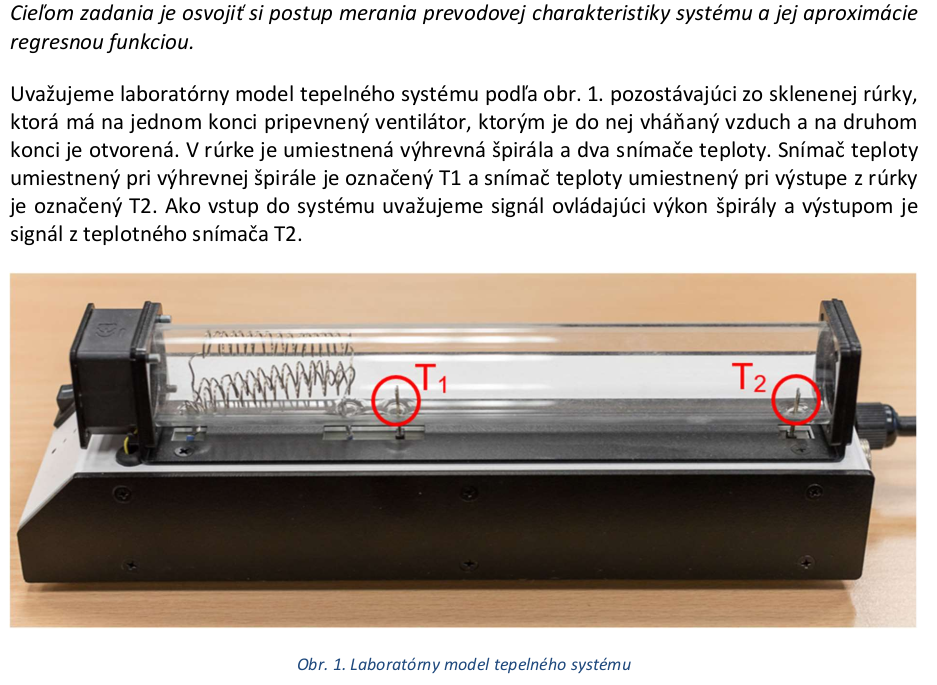
\includegraphics[width=0.8\textwidth]{./include/zadanie.png}
	\end{center}
	\caption{Zadania z~cvičenia č. 7 z~predmetu spojité procesy.}
	\label{fig:zadanie1}
\end{figure}

\clearpage

\section{Teória}
\label{sec:teoria}

Zadanie č. 7 sa zaoberá identifikáciou servosystému v~predurčenom pracovnom bode $U_0$.

\begin{figure}[!htbp]
	\begin{center}
		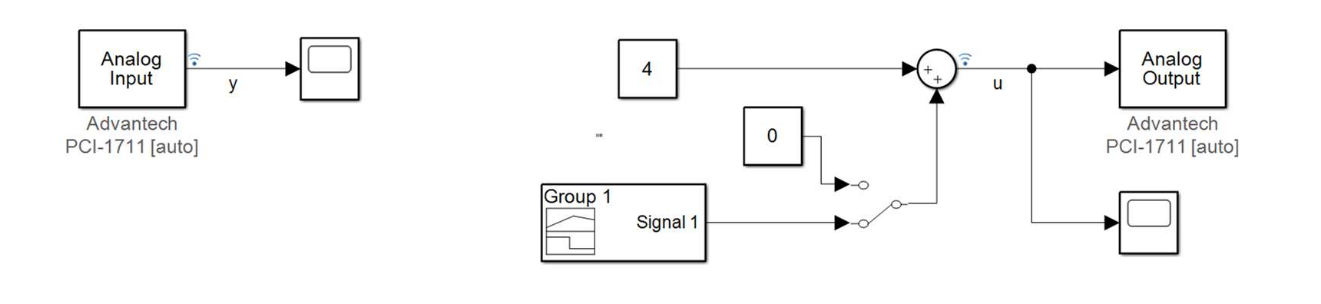
\includegraphics[width=0.95\textwidth]{include/schema.png}
	\end{center}
	\caption{Schéma zapojenia vstupu servosystému.}
	\label{fig:schema}
\end{figure}

Ako prvú vec si potrebujeme určiť hodnotu otáčok v~pracovnom bode. Ten máme preddefinovaný na~4V. Ako druhú vec budeme
zisťovať prenosovú funkciu, ktorá čo najpresnejšie opisuje nameraný graf. Vstupný signál pre~druhu úlohu vidíme na
obrázku.

\clearpage

\subsection{Uloha 1}
\label{subsec:u1}

Našou prvou úlohou ako už~bolo spomenuté v~\ref{sec:teoria} je nájsť pracovný bod. Predpísanú vstupnú hodnotu máme
$U_0 = 4V$. Tuto hodnotu sme mali už~prednastavenú v~simulácii \ref{fig:schema}. Simuláciu sme preto~spustili
a~odčítali sme ustálenú hodnotu z~grafu. Vstupný a~výstupný signál je zaznamenávaný s~periódou vzorkovania 0.01s.

Pri~vstupe $U_0 = 4V$ sme dostali na~výstupe rýchlosť otáčok $Y_0 = 6,8986$. Vstupný signál vidíme na~obrázku
Obr.~\ref{fig:uloha1_graf}

\begin{figure}[!htbp]
	\begin{center}
		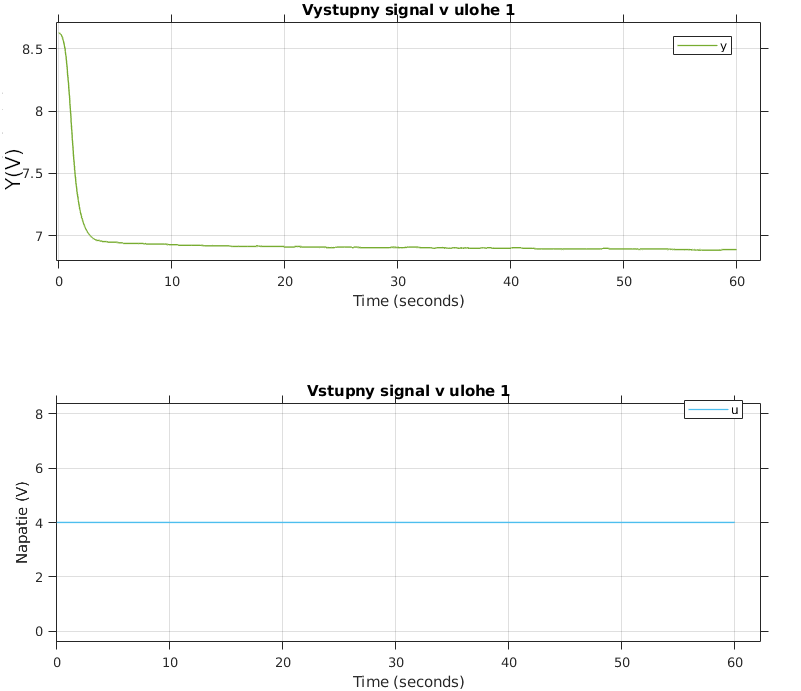
\includegraphics[width=0.95\textwidth]{include/uloha1_graf.png}
	\end{center}
	\caption{Vstupný a~výstupný signál prvej úlohy.}
	\label{fig:uloha1_graf}
\end{figure}

\clearpage

\section{Uloha 2}
\label{subsec:u2}

Na~začiatku druhej úlohy sme museli v~schéme prepnúť prepínač vstupného konštantného\\
signálu na~obdĺžnikový signál, ktorý sa pohybuje v~okolí pracovného bodu 4V s~amplitúdou 0.5V
(Obr.~\ref{fig:vstup2}). Perióda zmeny signálu je 10s. Podobne ako v~prvej úlohe,
perióda vzorkovania vstupného a~výstupného signálu je 0.01s.

\begin{figure}[!htbp]
	\begin{center}
		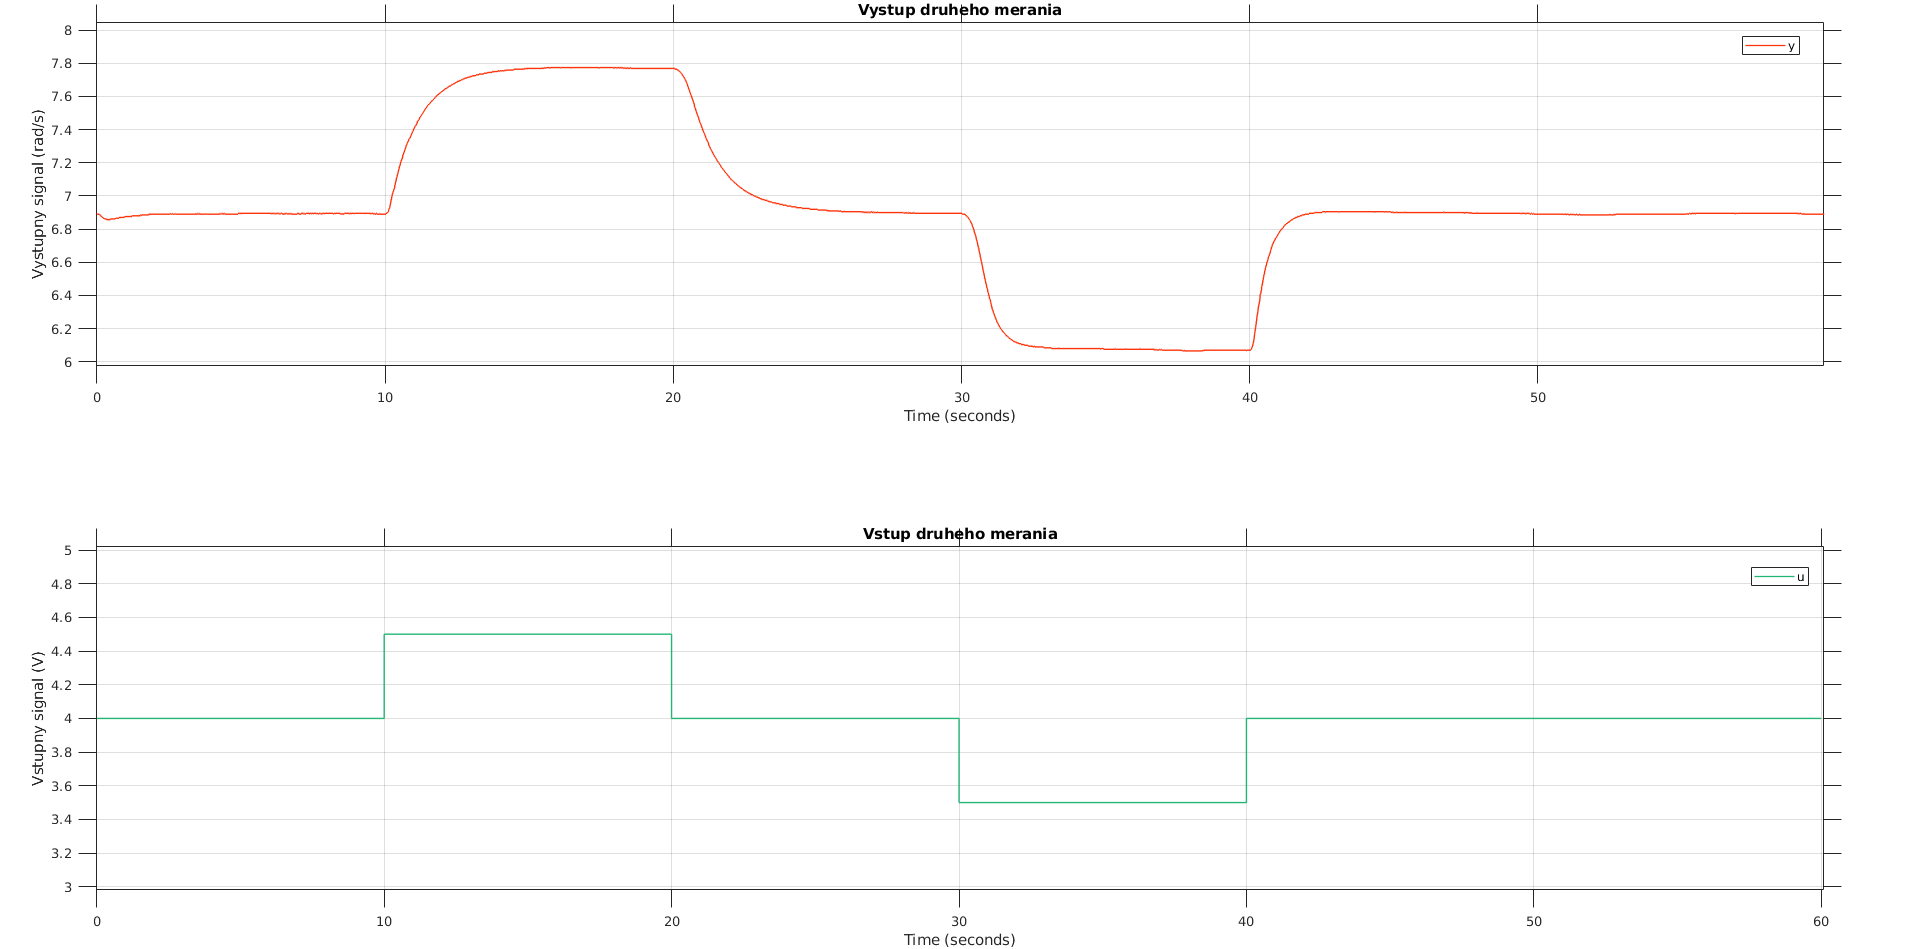
\includegraphics[width=0.95\textwidth]{include/vstup2_2.png}
	\end{center}
	\caption{Graf vstupného signálu do~servosystému v~úlohe 2.}
	\label{fig:vstup2}
\end{figure}

Identifikácia sa v~simulačnom prostredí MATLAB vykonáva pomocou funkcie \textbf{arx}.
Vstupne parametre tejto funkcie sú: 
\begin{itemize}
	\item matica vzorkovaných vstupno výstupných údajov
	\item vektor rádov
	\begin{itemize}
		\item čitateľa $n_a$
		\item menovateľa $n_b$
		\item dopravného oneskorenia $n_k$
	\end{itemize}
\end{itemize}

Aby sme zistili, ktorá identifikácia vychádza najlepšie. Počítame si sumu kvadrátu odchýliek medzi nameranou hodnotou
a~simulovanou hodnotou. Na~výpočet používame nasledovný vzťah:

\begin{equation}
	e = \sum_{i=0}^{i=N} (y_i - y_{si})^2
	\label{eq:odchylka}
\end{equation}
kde~$N$ je počet nameraných dát, $y$ sú~merane dáta a~$y_s$ sú~simulované dáta.

\clearpage

\subsection{Prvá identifikácia}
\label{subsec:I1}

Vstupné parametre rádov navrhovanej prenosovej funkcie sú:

\begin{lstlisting}[language=Matlab]
	na = 1;
	nb = 1;
	nk = 1;
\end{lstlisting}

\begin{figure}[!htbp]
	\begin{center}
		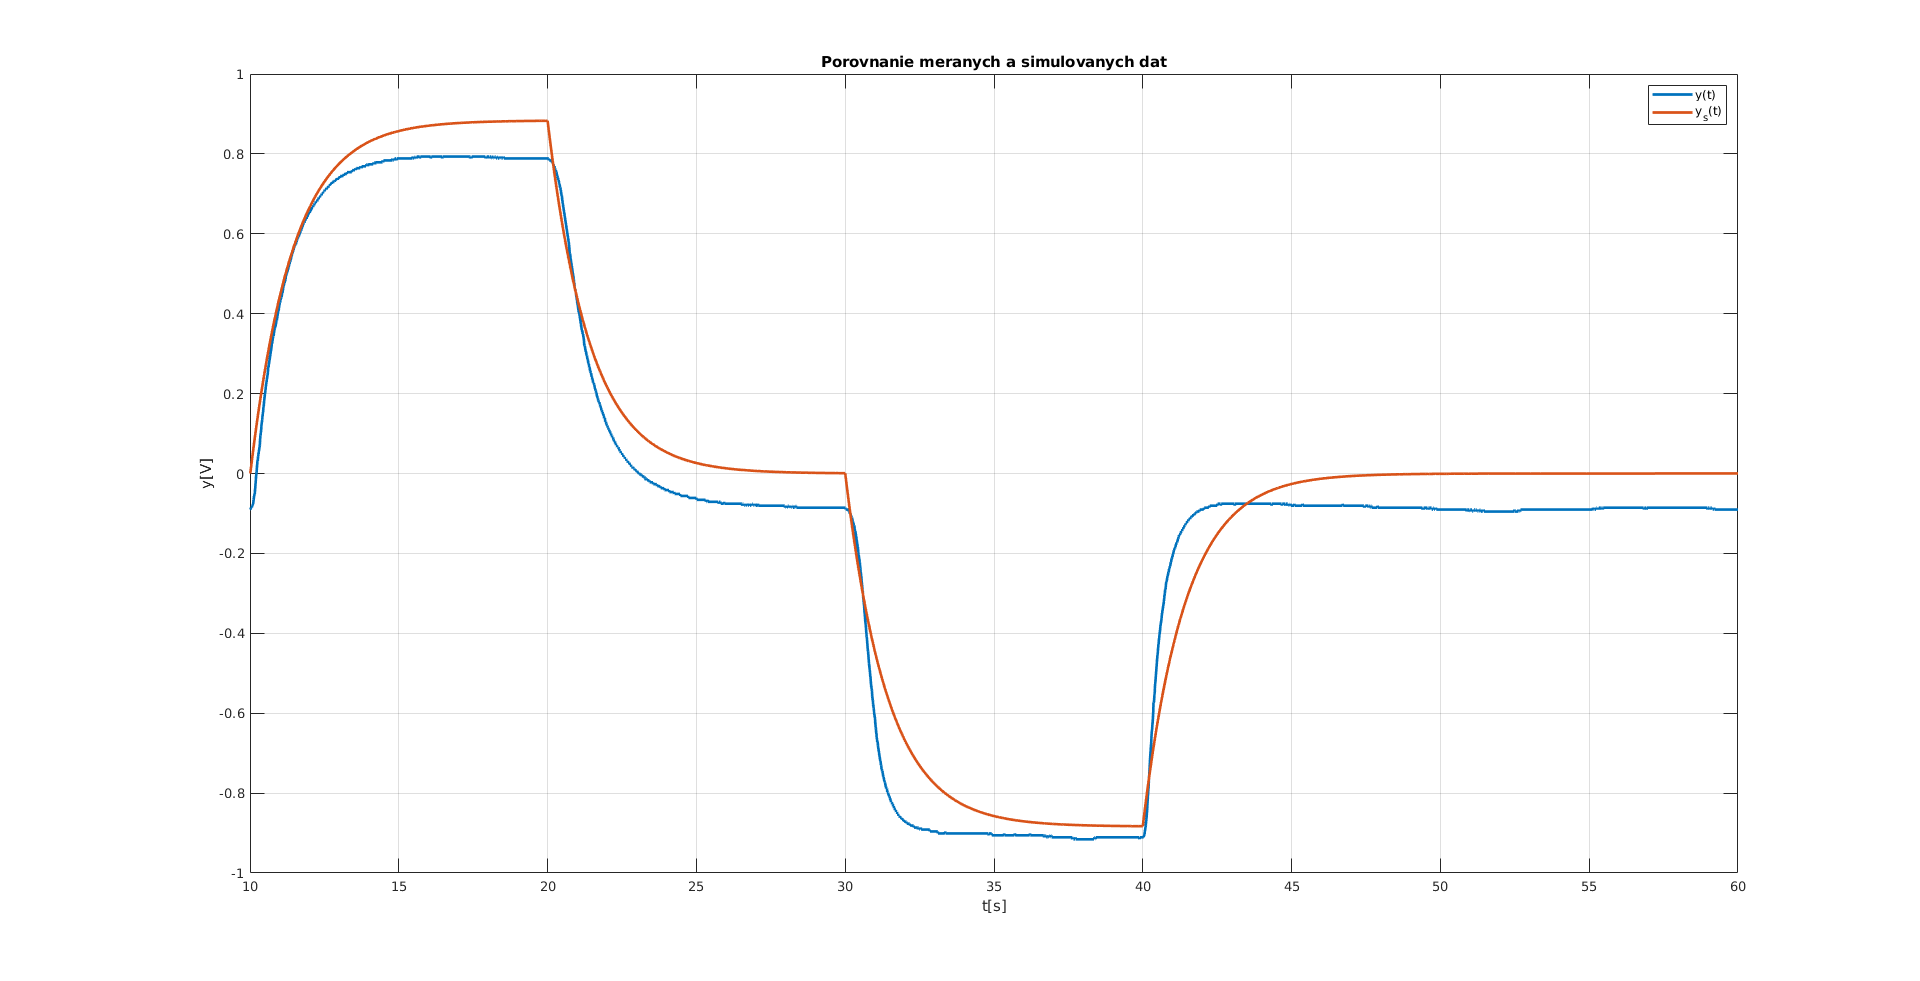
\includegraphics[width=0.95\textwidth]{include/I1.png}
	\end{center}
	\caption{Prvá identifikácia v~úlohe 2.}
	\label{fig:I1}
\end{figure}

Parametre pri~prvej identifikácii sme nastavili na~predvolené hodnoty a~to~$n_a = 1$, $n_b = 1$ a~$n_k = 1$.
Výsledná prenosová funkcia je:

\begin{equation}
	G_1(z) = \frac{0.01239}{z~- 0.993}
	\label{eq:I1}
\end{equation}

Odchýlka nám vyšla $e = 40.0690$

\clearpage

\end{document}

